\documentclass[11pt]{report}

%-------------------------------------------------------------------------------------------------%

% PAQUETES

\usepackage[a4paper, right = 0.8in, left = 0.8in, top = 0.8in, bottom = 0.8in]{geometry}
\usepackage[utf8]{inputenc}
\usepackage[spanish]{babel}
\usepackage{amsmath,amsfonts,amssymb,amsthm}
\usepackage{multicol}
\usepackage{fouriernc}
\usepackage{enumitem}
\usepackage{mathtools} % Solo uso \underbracket
\usepackage{cellspace, tabularx, booktabs} % Líneas del título
\usepackage{parskip}
\usepackage{pdfpages}
\usepackage{cancel}

%-------------------------------------------------------------------------------------------------%

% AJUSTES GENERALES

\setlist[enumerate]{label={\textit{\alph*})}}

\makeatletter % Para quitar el espacio adicional que el paquete parskip añade al principio y al final de una demostración
\renewenvironment{proof}[1][\proofname]{\par
  \pushQED{\qed}%
  \normalfont \topsep\z@skip % <---- changed here
  \trivlist
  \item[\hskip\labelsep
        \itshape
    #1\@addpunct{.}]\ignorespaces
}{%
  \popQED\endtrivlist\@endpefalse
}
\makeatother

%-------------------------------------------------------------------------------------------------%

% COMANDOS PERSONALIZADOS

\newcommand{\N}{\mathbb N}
\newcommand{\Z}{\mathbb Z}
\newcommand{\Q}{\mathbb Q}
\newcommand{\R}{\mathbb R}
\newcommand{\C}{\mathbb C}

\newcommand{\pars}[1]{\left( #1 \right)} % Paréntesis de tamaño automático
\newcommand{\comment}[1]{}

%-------------------------------------------------------------------------------------------------%

% EJERCICIOS Y SOLUCIONES

\newtheorem{ejercicio}{Ejercicio}
\addto\captionsspanish{\renewcommand*{\proofname}{Solución}}

%-------------------------------------------------------------------------------------------------%

\begin{document}

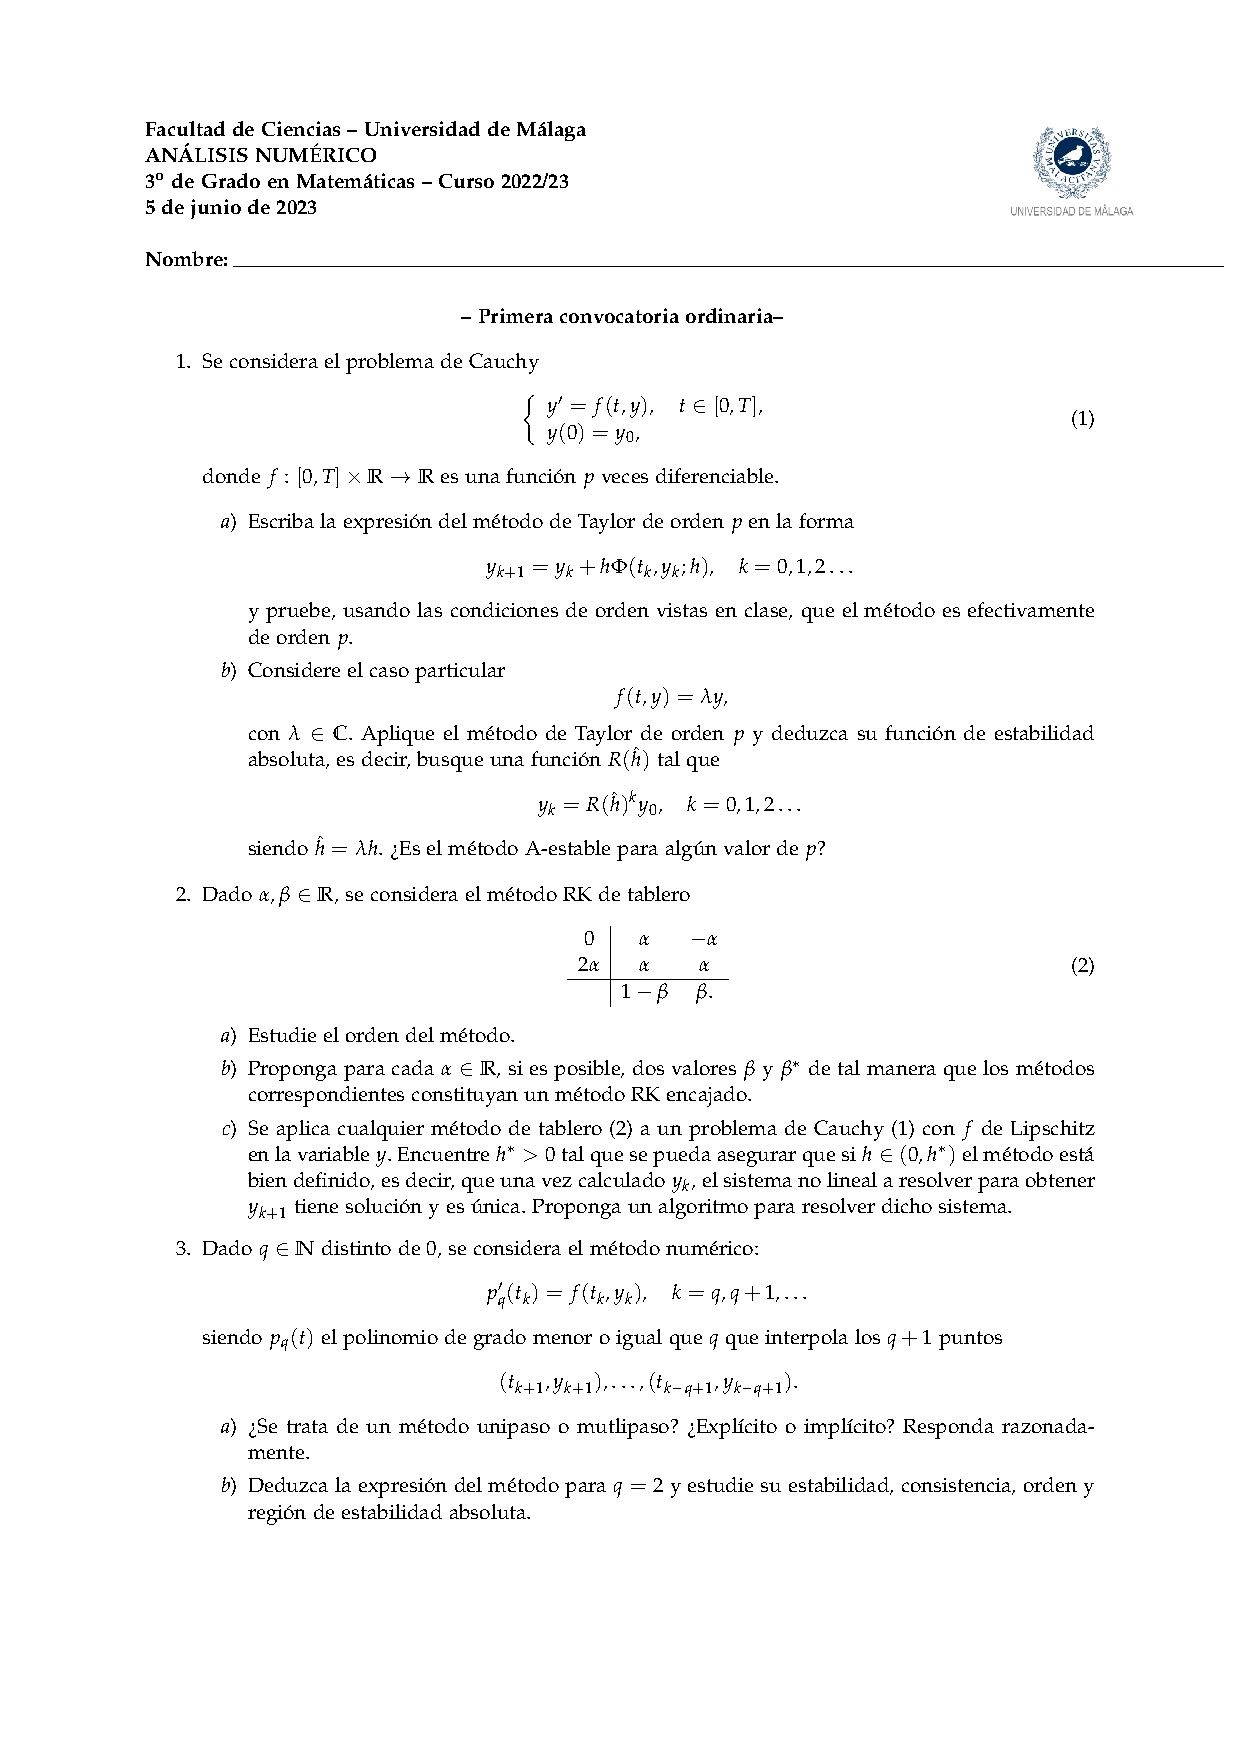
\includepdf[pages=-]{an_examen_2023-06.pdf}

%-------------------------------------------------------------------------------------------------%

% TÍTULO

\begin{center}

	\textbf{$-$ Resolución $-$}

\end{center}

%-------------------------------------------------------------------------------------------------%

\textbf{1.}

\begin{enumerate}
    \item El método de Taylor de orden $p$ es el método definido por 
    \[y_{k+1} = y_k+\sum_{i=1}^p \frac{f^{(i-1)}(t_k,y_k)}{i!}h^i, \qquad k =0,1,2,\mathellipsis\]
    donde, dado $n \in \N$, se define $f^{(n)}(t,y) \coloneqq f^{(n-1)}_t(t,y)+f(t,y)f^{(n)}_y(t,y)$ y para $n = 0$, $f^{(0)}(t,y)=f(t,y)$. El método de Taylor se puede escribir como
    \[y_{k+1} = y_k+h\sum_{i=1}^p \frac{f^{(i-1)}(t_k,y_k)}{i!}h^{i-1} =y_k+h\Phi(t_k,y_k,h), \qquad k =0,1,2,\mathellipsis\]
    donde
    \[\Phi(t,y,h) = \sum_{i=1}^p \frac{f^{(i-1)}(t,y)}{i!}h^{i-1} = \sum_{i=0}^{p-1}\frac{f^{(i)}(t,y)}{(i+1)!}h^i\]
    Veamos que el método es de orden $p$ o, equivalentemente, que para todo $j \in \{0,1,\mathellipsis,p-1\}$ se verifica
    \[\frac{\partial^j \Phi}{\partial h^j}(t,y,0) = \frac{1}{j+1}f^{(j)}(t,y) \tag{$\ast$}\]
    En $j = 0$,
    \[\frac{\partial^0 \Phi}{\partial h^0}(t,y,0) = \Phi(t,y,0) = \frac{f^{(0)}(t,y)}{0!} = f(t,y),\]
    así que se verifica la igualdad $(*)$. Para $j=1$,
    \[\frac{\partial \Phi}{\partial h} (t,y,h)=\sum_{i=1}^{p-1}\frac{i}{(i+1)!}f^{(i)}(t,y)h^{i-1}\]
    Poniendo $h=0$, el único sumando no nulo es el primero, así que
    \[\frac{\partial \Phi}{\partial h} (t,y,0)=\frac{1}{2}f^{(1)}(t,y)\]
    y también se da $(\ast)$. Hagámoslo también para $j = 2$:
    \[\frac{\partial^2\Phi}{\partial h^2}(t,y,h) = \sum_{i=2}^{p-1} \frac{i(i-1)}{(i+1)!}f^{(i)}(t,y)h^{i-2}\]
    Por tanto,
    \[\frac{\partial^2 \Phi}{\partial h^2}(t,y,0) = \frac{2 \cdot 1}{3!}f^{(2)}(t,y) = \frac{1}{3}f^{(2)}(t,y)\]
    Por inducción se prueba inmediatamente que para todo $j \in \in \{0,1,\mathellipsis,p-1\}$ se tiene
    \[\frac{\partial^j \Phi}{\partial h^j} (t,y,h) = \sum_{i=j}^{p-1}\frac{i(i-1)\mathellipsis(i-j+1)}{(i+1)!}f^{(i)}(t,y)h^{i-j}\]
    Por tanto, como en $h=0$ el único sumando no nulo es el de $i=j$, 
    \[\frac{\partial^j \Phi}{\partial h^j} (t,y,0)=\frac{j(j-1)\mathellipsis(j-j+1)}{(j+1)!}f^{(j)}(t,y) =  \frac{1}{j+1}f^{(j)}(t,y),\]
    así que también se verifica $(\ast)$ y por tanto el método es de orden $p$.
    \item Si $f(t,y)=\lambda y$, entonces
    \[f^{(1)}(t,y)=\cancel{f_t(t,y)}+f(t,y)f_y(t,y) = \lambda y \cdot \lambda = \lambda^2y\] 
    Además,
    \[f^{(2)}(t,y)=\cancel{f^{(1)}_t(t,y)}+f(t,y)f^{(1)}_y(t,y) =\lambda y \cdot \lambda^2 = \lambda^3y\]
    En general, se prueba fácilmente por inducción que
    \[f^{(i)}(t,y) = \lambda^{i+1}y\]
    para todo $i \in \{0,1,\mathellipsis,p-1\}$, luego el método de Taylor adopta la expresión
    \[
    \begin{aligned}[t]
    y_{k+1} = y_k+h\sum_{i=1}^p \frac{f^{(i-1)}(t_k,y_k)}{i!}h^{i-1} = y_k+h\sum_{i=1}^p \frac{\lambda^iy_k}{i!}h^{i-1} = y_k\left(1+\sum_{i=1}^p \frac{(\lambda h)^i}{i!}\right) = y_k\sum_{i=0}^p\frac{(\lambda h)^i}{i!}
    \end{aligned}
    \]
    Razonando por recurrencia,
    \[y_{k} = y_{k-1}\sum_{i=0}^p\frac{(\lambda h)^i}{i!}=y_{k-2}\left(\sum_{i=0}^p\frac{(\lambda h)^i}{i!}\right)^2 = \mathellipsis =y_0\left(\sum_{i=0}^p\frac{(\lambda h)^i}{i!}\right)^{k}\]
    Por tanto, la función de estabilidad absoluta del método es
    \[R(\hat{h}) = \sum_{i=0}^p \frac{\hat{h}^i}{i!}\]
    Nótese que el método de Taylor es un método RK explícito, así que no puede ser $A$-estable para ningún valor de $p$.
\end{enumerate}

\textbf{2.}

\begin{enumerate}
    \item Sean
    \[B = \left(\begin{array}{c}
        1-\beta \\
        \beta
    \end{array}\right)  \qquad E = \left(\begin{array}{c}
        1 \\
        1
    \end{array}\right) \qquad A = \left(\begin{array}{cc}
        \phantom{-}\alpha & -\alpha \\
        \phantom{-}\alpha & \phantom{-}\alpha 
    \end{array}\right) \qquad C=\left(\begin{array}{cc}
        0 & 0 \\
        0 & 2\alpha
    \end{array}\right)\]
    Estudiemos el orden del método. Se tiene que
    \[B^tE = \left(\begin{array}{cc}
        1-\beta & \beta
    \end{array}\right)\left(\begin{array}{c}
        1 \\
        1
    \end{array}\right) = 1-\beta+\beta = 1,\]
    así que el método es de orden $1$. Además,
    \[B^tAE = \left(\begin{array}{cc}
        1-\beta & \beta
    \end{array}\right)\left(\begin{array}{cc}
        \phantom{-}\alpha & -\alpha \\
        \phantom{-}\alpha & \phantom{-}\alpha 
    \end{array}\right)\left(\begin{array}{c}
        1 \\
        1
    \end{array}\right) =  \left(\begin{array}{cc}
        \alpha & 2\alpha\beta - \alpha
    \end{array}\right)\left(\begin{array}{c}
        1 \\
        1
    \end{array}\right) = 2\alpha\beta,\]
    así que el método es de orden $2$ si y solo si $2\alpha\beta = \frac{1}{2}$, es decir, si y solo si $\alpha\beta = \frac{1}{4}$. Más aún,
    \[
    \begin{aligned}[t]
    B^tC^2E &= \left(\begin{array}{cc}
        1-\beta & \beta
    \end{array}\right)\left(\begin{array}{cc}
        0 & 0 \\
        0 & 2\alpha
    \end{array}\right)\left(\begin{array}{cc}
        0 & 0 \\
        0 & 2\alpha
    \end{array}\right)\left(\begin{array}{c}
        1 \\
        1
    \end{array}\right) = \left(\begin{array}{cc}
        0 & 2\alpha\beta
    \end{array}\right)\left(\begin{array}{c}
        0 \\
        2\alpha
    \end{array}\right) = 2\alpha \cdot 2\alpha \beta \\
    B^tACE &= \left(\begin{array}{cc}
        1-\beta & \beta
    \end{array}\right)\left(\begin{array}{cc}
        \phantom{-}\alpha & -\alpha \\
        \phantom{-}\alpha & \phantom{-}\alpha 
    \end{array}\right)\left(\begin{array}{cc}
        0 & 0 \\
        0 & 2\alpha
    \end{array}\right)\left(\begin{array}{c}
        1 \\
        1
    \end{array}\right) = \left(\begin{array}{cc}
        \alpha & 2\alpha\beta - \alpha
    \end{array}\right)\left(\begin{array}{c}
        0 \\
        2\alpha
    \end{array}\right) = 2\alpha(2\alpha\beta-\alpha) \\
\end{aligned}
    \]
    El método será de orden $3$ si se verifican las siguientes condiciones:
    \[\left\{\begin{alignedat}{2}
        2\alpha\beta &=\frac{1}{2} \\[5pt]
        2\alpha \cdot 2\alpha\beta &=\frac{1}{3} \\[5pt]
        2\alpha(2\alpha\beta - \alpha) &= \frac{1}{6}
    \end{alignedat}
    \right. \quad \iff \quad \left\{\begin{alignedat}{2}
        2\alpha\beta &=\frac{1}{2} \\[5pt]
        2\alpha \cdot \frac{1}{2} &=\frac{1}{3} \\[5pt]
        2\alpha\left(\frac{1}{2} - \alpha\right) &= \frac{1}{6}
    \end{alignedat}
    \right. \quad \iff \quad \left\{\begin{alignedat}{2}
        2\alpha\beta &=\frac{1}{2} \\[5pt]
        \alpha &=\frac{1}{3} \\[5pt]
        \frac{2}{3}\left(\frac{1}{2} - \frac{1}{3}\right) &= \frac{1}{6}
    \end{alignedat}
    \right.\]
    Como la última ecuación no se verifica, concluimos que el método no es de orden $3$ para ningún valor de $\alpha$ y $\beta$, y es de orden $2$ si y solo si $\alpha\beta = \frac{1}{4}$.
    \item Los métodos encajados no entran este año.
    \item El método del enunciado viene dado por
    \[\left\{\begin{alignedat}{1}
        y_k^{(1)} &= y_k+h\bigl(\alpha f(t_k,y_k^{(1)}) -\alpha f(t_k+2\alpha h,y_k^{(2)})\bigr)\\
        y_k^{(2)} &= y_k+h\bigl(\alpha f(t_k,y_k^{(2)}) + \alpha f(t_k+2\alpha h, y_k^{(2)})\bigr) \\
        y_{k+1} &= y_k+h\bigl((1-\beta)f(t_k, y_k^{(1)})+\beta f(t_k+2\alpha h, y_k^{(2)})\bigr)
    \end{alignedat}\right.\]
    Para que el método esté bien definido, se necesita que el sistema
    \[(S) \ \left\{\begin{alignedat}{1}
        y_k^{(1)} &= y_k+h\bigl(\alpha f(t_k,y_k^{(1)}) -\alpha f(t_k+2\alpha h,y_k^{(2)})\bigr)\\
        y_k^{(2)} &= y_k+h\bigl(\alpha f(t_k,y_k^{(2)}) + \alpha f(t_k+2\alpha h, y_k^{(2)})\bigr) 
    \end{alignedat}\right.\]
    tenga una única solución. Esto equivale a que la función $G \colon \R^2 \to \R^2$ dada por
    \[G(Y) = G\left(\begin{array}{c}
        y^1 \\
        y^2
    \end{array}\right) = \left(\begin{array}{c}
        y_k+h\bigl(\alpha f(t_k,y^{1}) -\alpha f(t_k+2\alpha h,y^{2})\bigr) \\
        y_k+h\bigl(\alpha f(t_k,y^{1}) +\alpha f(t_k+2\alpha h,y^{2})\bigr)
    \end{array}\right)\]
    tenga un único punto fijo. El objetivo es tomar $h^*$ de manera que $G$ sea contractiva siempre que $h \in (0,h^*)$ y poder aplicar el teorema del punto fijo de Banach. Sean $Y,Z \in \R^2$. Entonces
    \[\begin{aligned}[t]
        |G_1(Y)-G_1(Z)| &= \left|\cancel{y_k}+h\bigl(\alpha f(t_k,y^{1}) -\alpha f(t_k+2\alpha h,y^{2})\bigr)-\cancel{y_k}-h\bigl(\alpha f(t_k,z^{1}) -\alpha f(t_k+2\alpha h,z^{2})\bigr)\right| \\
        &\leq h|\alpha| \left|f(t_k,y^1)-f(t_k,z^1)\right| + h |\alpha| \left|f(t_k+2\alpha h,z^2)-f(t_k+2\alpha h,y^2)\right| \\
        &\leq hL |\alpha| |y^1-z^1| + hL \alpha |y^2-z^2| \\
        &\leq 2hL|\alpha| ||Y-Z||_{\infty},
    \end{aligned}\]
    donde $L$ es la constante de Lipschitz de $f$. De forma totalmente análoga se prueba que
    \[|G_2(Y)-G_2(Z)| \leq 2hL |\alpha| ||Y-Z||_{\infty}\]
    Por tanto,
    \[||G(Y)-G(Z)||_{\infty} \leq 2hL|\alpha| ||Y-Z||_{\infty}\]
    Si tomamos el paso de malla de forma que se verifique
    \[0 < h < \frac{1}{2L|\alpha|}\]
    entonces se tendrá $2hL|\alpha|<1$, $G$ será contractiva y el teorema del punto fijo de Banach dirá que $G$ tiene un único punto fijo, lo que proporcionará una única solución para el sistema $(S)$ y asegurará la buena definición del método del enunciado. Por tanto, basta tomar
    \[h^*=\frac{1}{2L|\alpha|}\]
    Un algoritmo adecuado para resolver $(S)$ es el siguiente algoritmo de punto fijo:
    \[\begin{cases}
        Y_0 \in \R^2 \\
        Y_{n+1} = G(Y_n), \quad n =0,1,2,\mathellipsis
    \end{cases}\]
    El teorema del punto fijo de Banach también asegura que la sucesión dada por este método es convergente y su límite es el único punto fijo de $G$, que es la única solución del sistema $(S)$.
\end{enumerate}

\pagebreak

\textbf{3.}

\begin{enumerate}
    \item Se trata de un método multipaso, pues $p_q'(t_k)$ se calcula a partir de $y_{q+1},y_q,\mathellipsis,y_{1}$, es decir, para que el método arrance necesitan conocerse las $q+1$ primeras aproximaciones (y $q+1 >1$ porque $q \neq 0$). Concretamente, el método es de $q$ pasos, y como $p_q'(t_k)$ puede calcularse sin conocer $f_k$, el método es explícito.
    \item El método para $q = 2$ es
    \[p'(t_k) = f(t_k,y_k), \quad k = 2,3,\mathellipsis\]
    donde $p$ es el polinomio de grado menor o igual que $2$ que interpola los $3$ puntos
    \[(t_{k+1}, y_{k+1}),(t_{k}, y_{k}),(t_{k-1}, y_{k-1})\]
    La forma regresiva de Gregory-Newton para el polinomio de interpolación es
    \[p(t)=\widetilde{p}\left(\frac{t-t_{k+1}}{h}\right),\]
    donde
    \[\begin{aligned}[t]
        \widetilde{p}(s)&=\sum_{i=0}^2 \nabla^iy_{k+1} \binom{s+i-1}{i} = \nabla^0y_{k+1}\binom{s-1}{0}+\nabla^1y_{k+1}\binom{s}{1}+\nabla^2y_{k+1}\binom{s+1}{2} \\
        &= y_{k+1}+(y_{k+1}-y_k)s+\frac{1}{2}(y_{k+1}-2y_k+y_{k-1})s(s+1) \\
        &= y_{k+1}+(y_{k+1}-y_k)s+\frac{1}{2}(y_{k+1}-2y_k+y_{k-1})s^2+\frac{1}{2}(y_{k+1}-2y_k+y_{k-1})s \\
        &= y_{k+1}+\left(\frac{3}{2}y_{k+1}-2y_k+\frac{1}{2}y_{k-1}\right)s+\frac{1}{2}(y_{k+1}-2y_k+y_{k-1})s^2 \\
    \end{aligned}\]
    Se tiene que
    \[\widetilde{p}'(s)=\frac{3}{2}y_{k+1}-2y_k+\frac{1}{2}y_{k-1}+(y_{k+1}-2y_k+y_{k-1})s\]
    Por la regla de la cadena,
    \[p'(t)=\frac{1}{h}\widetilde{p}'\left(\frac{t-t_{k+1}}{h}\right)\]
    Por tanto,
    \[\begin{aligned}[t]
        p'(t_k)=\frac{1}{h}\widetilde{p}'\left(\frac{t_k-t_{k+1}}{h}\right) &= \frac{1}{h}\widetilde{p}'\left(-1\right) = \frac{1}{h}\left(\frac{3}{2}y_{k+1}-2y_k+\frac{1}{2}y_{k-1}-y_{k+1}+2y_k-y_{k-1}\right) \\ &= \frac{1}{h}\left(\frac{1}{2}y_{k+1}-\frac{1}{2}y_{k-1}\right)
     \end{aligned}\]
     La expresión del método es
     \[p'(t_k)=f(t_k,y_k), \quad k = 2,3,\mathellipsis\]
     es decir,
     \[\frac{1}{2}y_{k+1}-\frac{1}{2}y_{k-1} = hf_k, \quad k = 2,3,\mathellipsis\]
     Equivalentemente,
     \[\frac{1}{2}y_{k+2}-\frac{1}{2}y_{k} = hf_{k+1}, \quad k = 1,2,\mathellipsis\]
     Los polinomios característicos del método son 
     \[\rho(z)=\frac{1}{2}z^2-\frac{1}{2}, \qquad \qquad \sigma(z)=z\]
     Las raíces de $\rho$ son $1$ y $-1$, ambas de módulo $1$ y simples, así que el método es estable. Estudiemos el orden. Se tiene que
     \[\sum_{j=0}^2 \alpha_j = \frac{1}{2}-\frac{1}{2} = 0\]
     Además,
     \[\sum_{j=0}^2 \alpha_jj = \frac{1}{2} \cdot 2 = 1, \qquad \qquad \sum_{j=0}^2 \beta_j = 1\]
     Por tanto, el método es de orden $1$ (luego es consistente). De hecho,
     \[\sum_{j=0}^2\alpha_jj^2 = \frac{1}{2} \cdot 2^2 = 2, \qquad \qquad 2\sum_{j=0}^2 \beta_j j = 2 \cdot 1 = 2, \]
     así que el método es de orden $2$. Más aún,
     \[\sum_{j=0}^2 \alpha_jj^3 = \frac{1}{2}\cdot 2^3 = 4, \qquad \qquad 3\sum_{j=0}^2 \beta_jj^2 = 3 \cdot 1 = 3 \neq 4\]
     El método es de orden exactamente $2$. La frontera de la región de estabilidad absoluta es
     \[\partial D_A = \{\hat{h} \in \C \colon \pi_{\hat{h}} \textup{ tiene alguna raíz de módulo } 1\},\]
     donde $\pi_{\hat{h}}(z)=\rho(z)-\hat{h}\sigma(z)=\frac{1}{2}z^2-\hat{h}z-\frac{1}{2}$. Sea $\hat{h} \in \partial D_A$ y sea $e^{i\theta}$ una raíz de $\pi_{\hat{h}}$ de módulo $1$, con $\theta \in \R$. Entonces $\sigma(e^{i\theta}) = e^{i\theta} \neq 0$, así que
     \[\hat{h} = \frac{\rho(e^{i\theta})}{\sigma(e^{i\theta})} = \frac{\frac{1}{2}e^{2i\theta}-\frac{1}{2}}{e^{i\theta}} = \frac{1}{2}e^{i\theta}-\frac{1}{2}e^{-i\theta} =\frac{1}{2}2i\sen \theta = i\sen \theta\]
     Esto nos dice que $\partial D_A \subset \{iy \colon y \in [-1,1]\}$, así que hay dos posibilidades: $D_A = \C \setminus D_A$ o $D_A = \emptyset$. La primera opción es imposible porque $D_A$ no contiene a un intervalo de la forma $(0,\varepsilon)$ para algún $\varepsilon>0$, así que tiene que ser $D_A = \emptyset$.
\end{enumerate}

\end{document}
